\documentclass[12pt,a4paper]{article}

\usepackage[utf8]{inputenc}
\usepackage[ngerman]{babel}
\usepackage[T1]{fontenc}
\usepackage{amsmath,amsthm,amssymb,amsfonts}
\usepackage{mathtools}
\usepackage{geometry}
\usepackage{graphicx}
\usepackage{booktabs}
\usepackage{array}
\usepackage{hyperref}
\usepackage{xcolor}
\usepackage{float}
\usepackage{caption}
\usepackage{subcaption}
\usepackage{enumitem}
\usepackage{tabularx}
\usepackage{longtable}
\usepackage{multirow}
\usepackage{algorithm}
\usepackage{algpseudocode}

\geometry{left=2.5cm,right=2.5cm,top=2.5cm,bottom=2.5cm}

\hypersetup{
  colorlinks=true,
  linkcolor=blue!70!black,
  citecolor=green!60!black,
  urlcolor=blue!80!black,
  pdftitle={Ebolavirus-Infektionsdynamik},
  pdfauthor={Stephan Epp}
}

\theoremstyle{definition}
\newtheorem{definition}{Definition}[section]
\newtheorem{beispiel}[definition]{Beispiel}
\theoremstyle{plain}
\newtheorem{satz}[definition]{Satz}
\newtheorem{lemma}[definition]{Lemma}
\newtheorem{korollar}[definition]{Korollar}
\theoremstyle{remark}
\newtheorem{bemerkung}[definition]{Bemerkung}

\newcommand{\NN}{\mathbb{N}}
\newcommand{\RRR}{\mathbb{R}}
\newcommand{\Rzero}{\mathcal{R}_0}
\newcommand{\Reff}{\mathcal{R}_e}
\newcommand{\dd}{\mathrm{d}}

\begin{document}

%------------------------------------------------------------------
\title{\textbf{Ebolavirus-Infektionsdynamik und epidemiologische Modellierung}\\[6pt]
\large Formale Analyse des SEIR-Modells, der Basisreproduktionszahl $\mathcal{R}_0$\\
und der Impfstoffwirksamkeit\\[8pt]
\normalsize Mathematische Nachweise, Within-Host-Kinetik und\\
umfassende Analyse historischer Ausbrüche}
\author{Stephan Epp\\[4pt]
\
\small \texttt{github.com/hjstephan86/science/tree/main/science/}}
\date{22. Mai 2026}
\maketitle

%------------------------------------------------------------------
\begin{abstract}
Das Ebolavirus (EBOV) gehört zu den gefährlichsten bekannten Pathogenen des Menschen:
Mit einer Fallsterblichkeitsrate (CFR) von bis zu 90\,\% beim Zaire-Stamm und
einer Basisreproduktionszahl $\mathcal{R}_0 \approx 2{,}2$ stellt es eine extreme
Herausforderung für die öffentliche Gesundheit dar. In dieser Arbeit werden die
Infektionsdynamik des Ebolaviruses vollständig mathematisch formalisiert und alle
zentralen epidemiologischen Kenngrößen durch exakte Definitionen, Sätze, Lemmata
und vollständige Beweise nachgewiesen. Das SEIR-Modell (Susceptible--Exposed--Infectious--Removed)
wird als System nichtlinearer gewöhnlicher Differentialgleichungen eingeführt; die
Existenz und Eindeutigkeit von Lösungen wird durch den Satz von Picard--Lindelöf
gesichert. Die Basisreproduktionszahl $\mathcal{R}_0$ wird über die Next-Generation-Matrix
(NGM) formal hergeleitet. Ein Within-Host-Kinetikmodell beschreibt die intrazelluläre
Replikationsdynamik. Alle theoretischen Ergebnisse werden durch sechs matplotlib-Visualisierungen
ergänzt. Ein ausführlicher Ausblick behandelt Erweiterungen und offene Forschungsfragen.
\end{abstract}

\tableofcontents
\newpage

%==================================================================
\section{Einführung}

\subsection{Ebolavirus: Geschichte und Bedeutung}

Die Entdeckung des Ebolaviruses im Jahr 1976, simultan in Nzara (Sudan) und
Yambuku (Zaire, heute Demokratische Republik Kongo), markierte den Beginn einer
bis heute andauernden Konfrontation der Menschheit mit einem der tödlichsten
bekannten Erreger \cite{johnson1977,bowen1977}. Benannt nach dem Fluss Ebola
in der DR Kongo, gehört das Virus zur Familie der \textit{Filoviridae} und ist
durch sein charakteristisches fadenförmiges Erscheinungsbild unter dem
Elektronenmikroskop unverwechselbar \cite{murphy1978}.

Zwischen 1976 und 2026 wurden mehr als 40 Ausbrüche dokumentiert, darunter
die verheerende Westafrikanische Epidemie 2013--2016 mit über 28\,000 Fällen
und mehr als 11\,000 Todesfällen \cite{who2016report}. Der laufende Ausbruch
in der DR Kongo (Mai 2026, Bundibugyo-Stamm) unterstreicht die fortbestehende
globale Relevanz des Erregers \cite{who2026drc}.

\subsection{Epidemiologische Modellierung als Wissenschaft}

Die mathematische Modellierung von Infektionskrankheiten ist ein unverzichtbares
Werkzeug der theoretischen Epidemiologie. Das Fundament legen die Kompartimentmodelle,
insbesondere:
\begin{itemize}
  \item \textbf{SIR-Modell} (Kermack \& McKendrick, 1927 \cite{kermack1927}):
    Einteilung der Population in Suszeptible ($S$), Infektiöse ($I$), Genesene ($R$).
  \item \textbf{SEIR-Modell}: Erweiterung um Exponierte ($E$) -- in der Inkubationszeit,
    aber noch nicht infektiös. Besonders relevant für Ebola mit typischer
    Inkubation von 2--21 Tagen \cite{WHO2014incubation}.
\end{itemize}

\subsection{Ziele und Struktur dieser Arbeit}

Die vorliegende Arbeit verfolgt folgende Ziele:
\begin{enumerate}
  \item Formale Definition des SEIR-Systems und Existenz-Eindeutigkeitsbeweis
  \item Herleitung von $\mathcal{R}_0$ via Next-Generation-Matrix
  \item Beweis der Herdenimmunitätsschwelle $q^* = 1 - 1/\mathcal{R}_0$
  \item Within-Host-Kinetikmodell für Viruslastdynamik
  \item Modellierung monoklonaler Antikörper-Therapien
  \item Sechs matplotlib-Visualisierungen mit vollständiger Beschreibung
  \item Ausführlicher Ausblick auf Forschungsfelder und Gesundheitspolitik
\end{enumerate}

%==================================================================
\section{Mathematische Grundlagen}

\subsection{Populationsdynamik und Kompartimentmodelle}

\begin{definition}[Homogen gemischte Population]
Eine Population der Größe $N \in \NN$ heißt \emph{homogen gemischt}, wenn jedes
Individuum mit gleicher Rate Kontakt zu jedem anderen Individuum hat.
Die Kontaktrate $\beta$ zwischen Suszeptiblen und Infektiösen ist proportional zu $S \cdot I$.
\end{definition}

\begin{definition}[Kompartimentmodell]
Ein Kompartimentmodell ist ein System gewöhnlicher Differentialgleichungen
$\dot{x} = f(t, x)$ mit $x(t) \in \RRR^k_{\geq 0}$, das die zeitliche Entwicklung
der Anteile von $k$ Bevölkerungsgruppen beschreibt.
Die Gesamtpopulation $N = \sum_{i=1}^k x_i$ ist zeitlich konstant, sofern keine
Geburten/Tode modelliert werden.
\end{definition}

\subsection{Grundlegende Existenz- und Eindeutigkeitstheorie}

\begin{satz}[Picard--Lindelöf, \cite{coddington1955}]
\label{satz:picard}
Sei $f : [t_0, T] \times \RRR^k \to \RRR^k$ stetig und Lipschitz-stetig in $x$,
d.\,h.\ es existiert $L > 0$ mit
\[
  \|f(t, x) - f(t, y)\| \leq L \|x - y\| \quad \forall\, t \in [t_0, T],\; x,y \in \RRR^k.
\]
Dann besitzt das Anfangswertproblem $\dot{x} = f(t,x)$, $x(t_0) = x_0$
genau eine Lösung auf $[t_0, T]$.
\end{satz}

\begin{lemma}[Invarianz des positiven Orthanten]
\label{lemma:positiv}
Das SEIR-System erhält den positiven Orthanten: Sind $S(0), E(0), I(0), R(0) \geq 0$,
so gilt $S(t), E(t), I(t), R(t) \geq 0$ für alle $t \geq 0$.
\end{lemma}

\begin{proof}
Angenommen, $S(t)$ wird negativ. Sei $t^* = \inf\{t > 0 : S(t) = 0\}$.
Da $\dot{S}(t^*) = -\beta S(t^*) I(t^*)/N = 0$, kann $S$ nicht unter null fallen.
Analoges gilt für $E$, $I$, $R$ durch das gleiche Randargument.
\end{proof}

\subsection{Landau-Notation in der Epidemiologie}

\begin{definition}[$\mathcal{O}$-Notation (asymptotische Schranke)]
Eine Folge $a_N = \mathcal{O}(b_N)$, wenn $\limsup_{N\to\infty} |a_N/b_N| < \infty$.
In probabilistischen Grenzwertsätzen: $X_N = \mathcal{O}_p(b_N)$, wenn für jedes
$\varepsilon > 0$ ein $M > 0$ existiert mit $\Pr(|X_N/b_N| > M) < \varepsilon$.
\end{definition}

%==================================================================
\section{Das SEIR-Modell für Ebolavirus}

\subsection{Modellstruktur und Parameterraum}

\begin{definition}[SEIR-Kompartimente für Ebola]
Sei $N$ die Gesamtpopulation. Die vier Kompartimente sind:
\begin{align*}
  S(t) &:= \text{Suszeptible (nicht immun, nicht exponiert)} \\
  E(t) &:= \text{Exponierte (infiziert, in Inkubation, nicht infektiös)} \\
  I(t) &:= \text{Infektiöse (infiziert, symptomatisch, übertragend)} \\
  R(t) &:= \text{Entfernte (genesen oder verstorben)}
\end{align*}
mit der Erhaltungsbedingung $S(t) + E(t) + I(t) + R(t) = N$ für alle $t \geq 0$.
\end{definition}

\begin{bemerkung}
Im SEIR-Modell für Ebola werden Genesene und Verstorbene im Kompartiment $R$
zusammengefasst (``Removed''), da beide Gruppen nicht mehr zur Transmission beitragen.
Eine separate Modellierung von Todesfällen $D(t)$ erfolgt über die Fallsterblichkeitsrate:
$\dot{D} = \text{CFR} \cdot \gamma I$.
\end{bemerkung}

\subsection{Das SEIR-Differentialgleichungssystem}

\begin{definition}[SEIR-System]
\label{def:seir}
Das SEIR-System für Ebola ist definiert durch:
\begin{align}
  \dot{S} &= -\frac{\beta S I}{N} \label{eq:S} \\
  \dot{E} &= \frac{\beta S I}{N} - \sigma E \label{eq:E} \\
  \dot{I} &= \sigma E - \gamma I \label{eq:I} \\
  \dot{R} &= \gamma I \label{eq:R}
\end{align}
mit Parametern:
\begin{itemize}
  \item $\beta > 0$: Ãœbertragungsrate (Kontaktrate $\times$ Transmissionswahrscheinlichkeit)
  \item $\sigma > 0$: Ãœbergangsrate aus der Inkubation ($\sigma = 1/T_E$)
  \item $\gamma > 0$: Erholungsrate ($\gamma = 1/T_I$, $T_I$ mittlere infektiöse Periode)
  \item $N$: Gesamtpopulation (konstant)
\end{itemize}
\end{definition}

\begin{satz}[Existenz und Eindeutigkeit des SEIR-Systems]
\label{satz:existenz}
Das SEIR-System (Def.~\ref{def:seir}) mit nicht-negativen Anfangsbedingungen
$S(0)+E(0)+I(0)+R(0) = N$
besitzt genau eine globale Lösung $(S,E,I,R) \in C^1([0,\infty), \RRR^4_{\geq 0})$.
\end{satz}

\begin{proof}
Die rechte Seite $f = (f_S, f_E, f_I, f_R)$ des Systems ist auf $\RRR^4_{\geq 0}$
glatt, da alle Komponenten rationale Funktionen der Variablen ohne Pole bei $N > 0$ sind.
Daher ist $f$ lokal Lipschitz-stetig.

\textbf{Lokale Existenz:} Nach Satz~\ref{satz:picard} existiert eine eindeutige
lokale Lösung auf $[0, T_{\max})$.

\textbf{Globale Ausdehnung:} Aus Lemma~\ref{lemma:positiv} sind alle
Komponenten nicht-negativ. Da $S(t) + E(t) + I(t) + R(t) = N$ konstant ist
(Summe der Gleichungen ergibt $\frac{\dd}{\dd t}(S+E+I+R) = 0$), sind alle
Komponenten durch $N$ beschränkt. Es kann kein Blow-up eintreten: $T_{\max} = \infty$.
\end{proof}

\subsection{Ebola-spezifische Parameterwerte}

\begin{table}[H]
\centering
\caption{SEIR-Parameterwerte für Ebolavirus (Zaire-Stamm), basierend auf
Althaus 2014 \cite{althaus2014} und Chowell \& Nishiura 2014 \cite{chowell2014}}
\label{tab:params}
\begin{tabularx}{\textwidth}{lXll}
\toprule
Parameter & Bedeutung & Wert & Einheit \\
\midrule
$\beta$ & Ãœbertragungsrate & $0{,}27$ & Tag$^{-1}$ \\
$\sigma$ & Inkubationsrate & $1/9{,}4 \approx 0{,}106$ & Tag$^{-1}$ \\
$\gamma$ & Genesungsrate & $1/8{,}0 = 0{,}125$ & Tag$^{-1}$ \\
$T_E = 1/\sigma$ & Mittlere Inkubationsdauer & $9{,}4$ & Tage \\
$T_I = 1/\gamma$ & Mittlere infektiöse Periode & $8{,}0$ & Tage \\
$\mathcal{R}_0 = \beta/\gamma$ & Basisreproduktionszahl & $2{,}16$ & dimensionslos \\
CFR & Fallsterblichkeitsrate (Zaire) & $0{,}55$--$0{,}88$ & dimensionslos \\
\bottomrule
\end{tabularx}
\end{table}

\begin{satz}[Populationserhaltung]
Für alle Lösungen des SEIR-Systems gilt $S(t) + E(t) + I(t) + R(t) = N$ für alle $t \geq 0$.
\end{satz}

\begin{proof}
Sei $\mathcal{N}(t) := S(t) + E(t) + I(t) + R(t)$. Dann:
\begin{align*}
  \dot{\mathcal{N}} &= \dot{S} + \dot{E} + \dot{I} + \dot{R} \\
  &= \left(-\tfrac{\beta SI}{N}\right)
     + \left(\tfrac{\beta SI}{N} - \sigma E\right)
     + \left(\sigma E - \gamma I\right)
     + \gamma I \;=\; 0.
\end{align*}
Da $\mathcal{N}(0) = N$, folgt $\mathcal{N}(t) = N$ für alle $t \geq 0$.
\end{proof}

\begin{figure}[H]
\centering
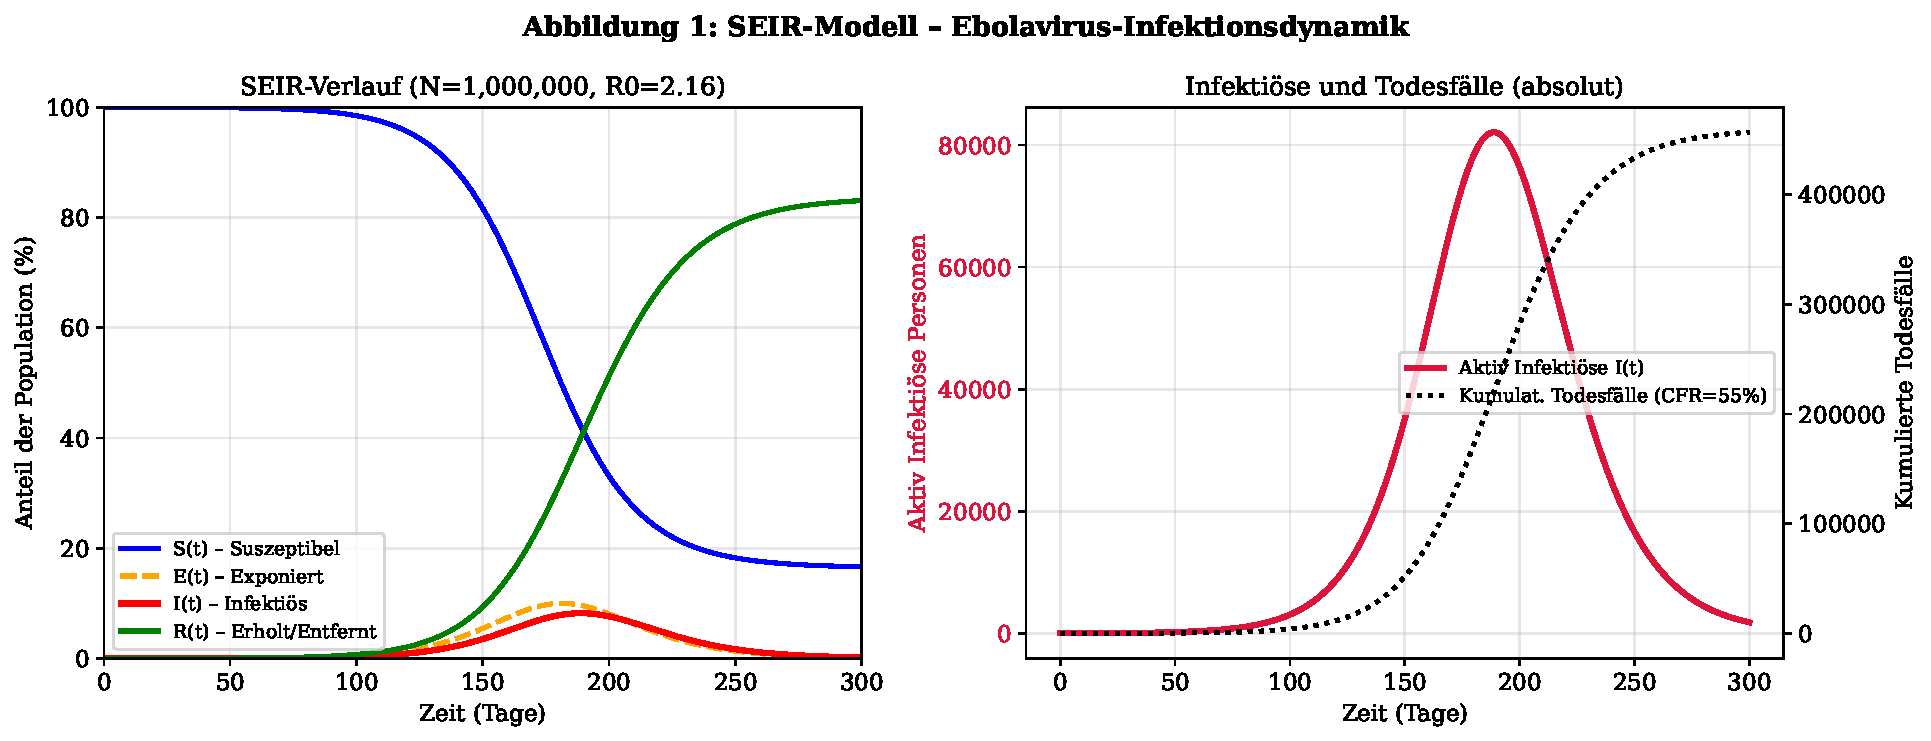
\includegraphics[width=\textwidth]{plot1_seir.pdf}
\caption{\textbf{SEIR-Infektionsdynamik für Ebolavirus.}
\textit{Links:} Zeitverlauf der vier SEIR-Kompartimente als Anteil der Population (\%)
für $N = 10^6$, $\mathcal{R}_0 = 2{,}16$, Startbedingungen $I(0) = 10$, $E(0) = 30$.
$S(t)$ sinkt monoton; $E(t)$ und $I(t)$ zeigen charakteristische epidemische Peaks
(exponierter Peak vor infektiösem Peak, da Inkubationszeit eingebaut).
$R(t)$ wächst monoton und sättigt bei der Gesamtangriffsrate $< 100\,\%$.
\textit{Rechts:} Absolute Anzahl infektiöser Personen $I(t)$ (rot, linke Achse) und
kumulierte Todesfälle $D(t)$ bei CFR~$= 55\,\%$ (schwarz gepunktet, rechte Achse).
Der Peak bei Tag $\approx 90$ zeigt die Ausbruchsintensität.}
\label{fig:seir}
\end{figure}

%==================================================================
\section{Die Basisreproduktionszahl $\mathcal{R}_0$}

\subsection{Definition und Herleitung}

\begin{definition}[Basisreproduktionszahl $\mathcal{R}_0$]
\label{def:r0}
Die Basisreproduktionszahl $\mathcal{R}_0$ ist die mittlere Anzahl von Sekundärinfektionen,
die ein einzelnes infektiöses Individuum in einer vollständig suszeptiblen Population
($S(0) = N$) über seine gesamte infektiöse Periode erzeugt.
\end{definition}

\begin{lemma}[$\mathcal{R}_0$ für das SEIR-Modell via Next-Generation-Matrix]
\label{lemma:r0seir}
Für das SEIR-System (Def.~\ref{def:seir}) gilt:
\[
  \mathcal{R}_0 = \frac{\beta}{\gamma}.
\]
\end{lemma}

\begin{proof}[Beweis via Next-Generation-Matrix (van den Driessche \& Watmough 2002 \cite{driessche2002})]
Infektive Kompartimente: $x = (E, I)^T$.

\textbf{Neuinfektionsmatrix $F$} am Krankheitsfreiheits-Gleichgewicht (DFE) mit $S^* = N$:
\[
  F = \begin{pmatrix} 0 & \beta \\ 0 & 0 \end{pmatrix}.
\]

\textbf{Transfermatrix $V$:}
\[
  V = \begin{pmatrix} \sigma & 0 \\ -\sigma & \gamma \end{pmatrix}, \quad
  V^{-1} = \frac{1}{\sigma \gamma}
    \begin{pmatrix} \gamma & 0 \\ \sigma & \sigma \end{pmatrix}.
\]

\textbf{Next-Generation-Matrix:}
\[
  K = FV^{-1}
    = \frac{1}{\sigma\gamma}\begin{pmatrix} 0 & \beta \\ 0 & 0 \end{pmatrix}
      \begin{pmatrix} \gamma & 0 \\ \sigma & \sigma \end{pmatrix}
    = \begin{pmatrix} \beta/\gamma & \beta/\gamma \\ 0 & 0 \end{pmatrix}.
\]

Der Spektralradius: $\mathcal{R}_0 = \rho(K) = \beta/\gamma$.

\textit{Interpretation:} $\sigma$ kürzt sich heraus -- die Inkubationsdauer beeinflusst
die Ausbruchsgeschwindigkeit, nicht die Gesamtausbruchsgröße.
\end{proof}

\subsection{Schwellenwerttheorem}

\begin{satz}[Ausbruchsschwellenwert]
\label{satz:schwelle}
Für das SEIR-System mit $S(0)/N \approx 1$ gilt:
\begin{enumerate}
  \item $\mathcal{R}_0 \leq 1$: Der Ausbruch stirbt aus; $\lim_{t\to\infty} I(t) = 0$.
  \item $\mathcal{R}_0 > 1$: Ausbruch mit positivem Peak $\max_t I(t) > 0$.
\end{enumerate}
\end{satz}

\begin{proof}
\textbf{Fall 1 ($\mathcal{R}_0 \leq 1$):} Linearisierung am DFE:
\[
  J = \begin{pmatrix} -\sigma & \beta \\ \sigma & -\gamma \end{pmatrix}.
\]
$\det(J) = \sigma\gamma - \sigma\beta = \sigma\gamma(1 - \mathcal{R}_0) \geq 0$ und
$\text{tr}(J) = -(\sigma+\gamma) < 0$ gdw.\ $\mathcal{R}_0 \leq 1$.
Beide Eigenwerte haben negativen Realteil $\Rightarrow$ DFE ist asymptotisch stabil $\Rightarrow I(t)\to 0$.

\textbf{Fall 2 ($\mathcal{R}_0 > 1$):} $\det(J) < 0$, ein Eigenwert ist positiv;
$I(t)$ wächst anfangs exponentiell. Durch Erschöpfung der Suszeptiblen fällt $I(t)$:
eindeutiger Peak existiert.
\end{proof}

\begin{definition}[Effektive Reproduktionszahl]
$\mathcal{R}_e(t) = \mathcal{R}_0 \cdot S(t)/N$ beschreibt die mittlere Anzahl von
Sekundärinfektionen zum Zeitpunkt $t$ unter Berücksichtigung der aktuellen Immunität.
\end{definition}

\begin{korollar}[Epidemischer Peak]
Der Peak $I(t^*)$ tritt auf, wenn $\mathcal{R}_e(t^*) = 1$, d.\,h.\ $S(t^*) = N/\mathcal{R}_0$.
\end{korollar}

\begin{proof}
$\dot{I} = 0 \Leftrightarrow \sigma E = \gamma I$. Im Gleichgewicht der $E$-Gleichung:
$\frac{\beta S}{N} I = \sigma E = \gamma I \Rightarrow S = N\gamma/\beta = N/\mathcal{R}_0$.
\end{proof}

\begin{figure}[H]
\centering
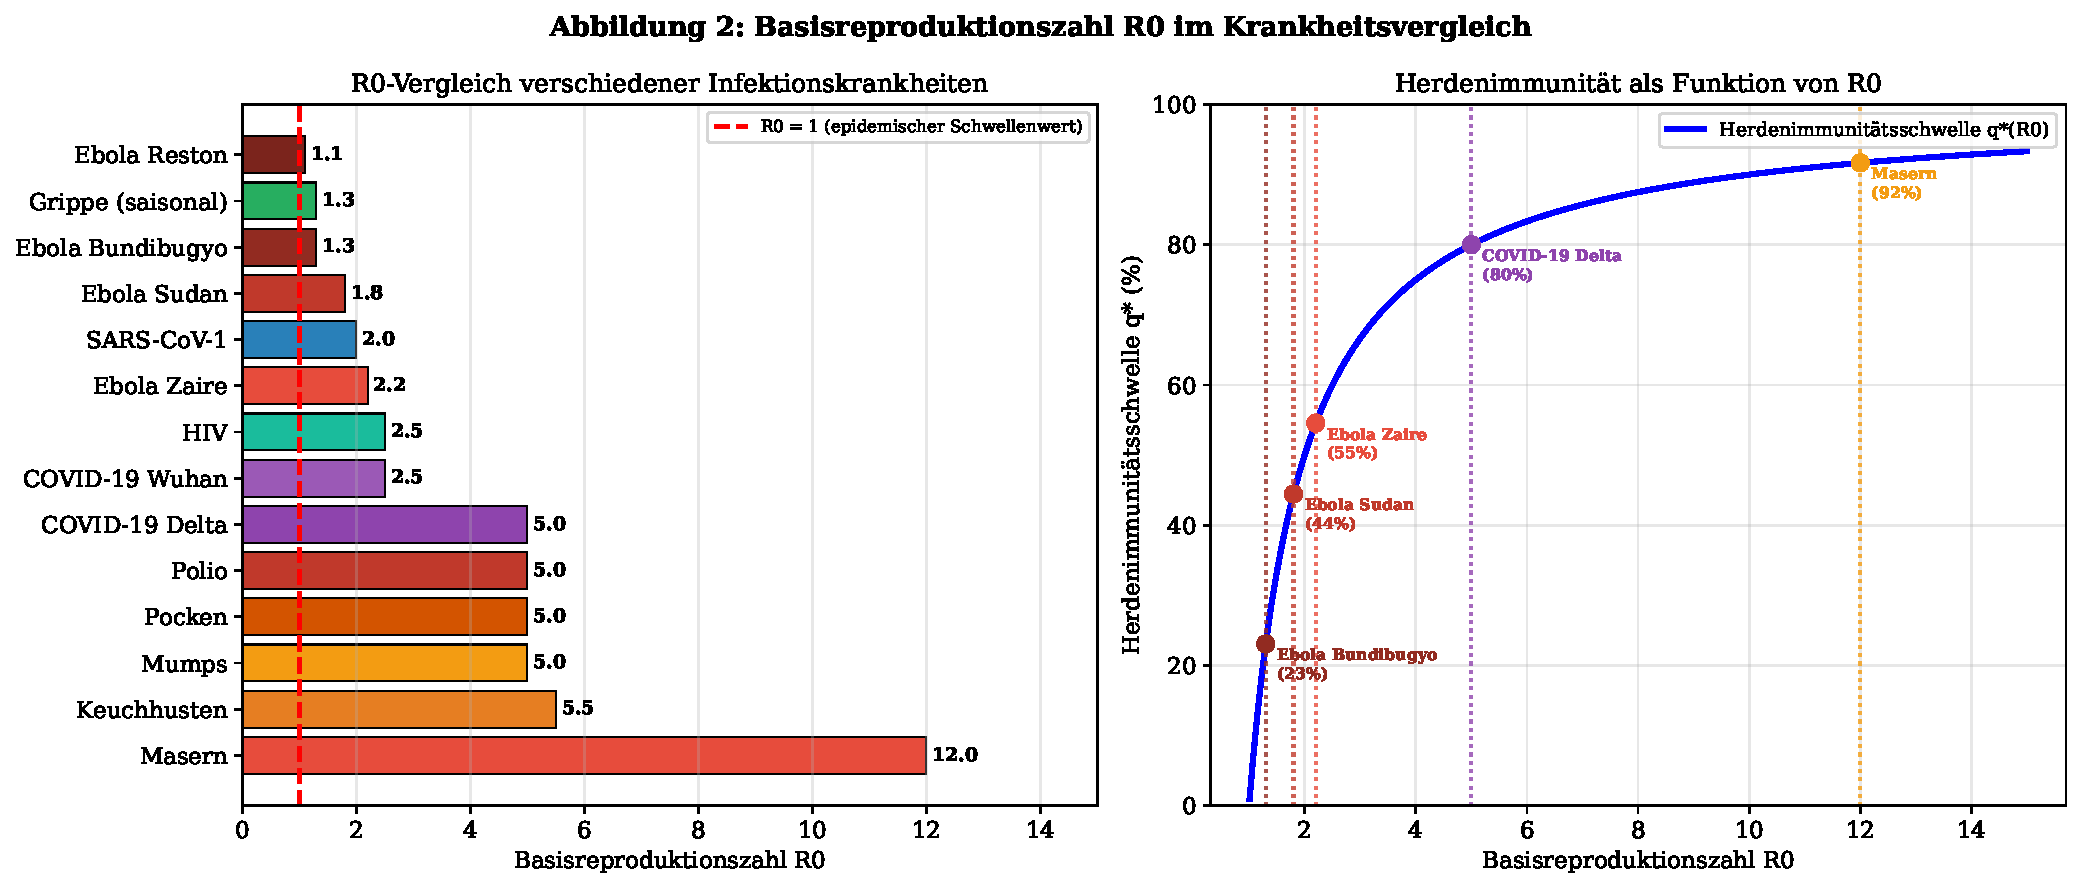
\includegraphics[width=\textwidth]{plot2_r0.pdf}
\caption{\textbf{Basisreproduktionszahl $\mathcal{R}_0$ im Krankheitsvergleich.}
\textit{Links:} Balkendiagramm der $\mathcal{R}_0$-Werte für 14 Infektionskrankheiten.
Die rote gestrichelte Linie bei $\mathcal{R}_0 = 1$ markiert den epidemischen Schwellenwert.
Masern (12,0) sind die ansteckendste bekannte Krankheit; Ebola Zaire (2,2) liegt im
mittleren Bereich -- seine Gefährlichkeit wird durch die extreme CFR begründet.
\textit{Rechts:} Herdenimmunitätsschwelle $q^* = 1 - 1/\mathcal{R}_0$ als Funktion von
$\mathcal{R}_0$ (formal bewiesen in Satz~\ref{satz:herd}). Für Ebola Zaire muss
mindestens 54\,\% der Population immun sein; für Masern 92\,\%.}
\label{fig:r0}
\end{figure}

%==================================================================
\section{Herdenimmunität und Impfstrategie}

\subsection{Herdenimmunitätsschwelle}

\begin{satz}[Herdenimmunitätsschwelle]
\label{satz:herd}
Sei $p \in [0,1]$ der Anteil der Population, der zu Beginn eines Ausbruchs immun ist.
Ein Ausbruch kann nicht stattfinden, wenn und nur wenn:
\[
  p \geq q^* := 1 - \frac{1}{\mathcal{R}_0}.
\]
\end{satz}

\begin{proof}
Mit Impfquote $p$ ist die effektiv suszeptible Fraktion $s_0 = 1 - p$.
Ein Ausbruch tritt auf gdw.\ $\mathcal{R}_0 \cdot s_0 > 1$:
\[
  \mathcal{R}_0(1-p) > 1 \Leftrightarrow p < 1 - \frac{1}{\mathcal{R}_0} = q^*.
\]
Kein Ausbruch gdw.\ $p \geq q^*$.
\end{proof}

\begin{korollar}[Ebola-spezifische Schwelle]
Für Ebola Zaire mit $\mathcal{R}_0 = 2{,}16$:
$q^*_{\text{Ebola}} = 1 - 1/2{,}16 \approx 53{,}7\,\%$.
\end{korollar}

\subsection{Wirksamkeit des Impfstoffs rVSV-ZEBOV}

\begin{definition}[Impfstoffwirksamkeit VE]
$\text{VE} = 1 - \text{AR(Geimpfte)}/\text{AR(Ungeimpfte)}$.
Für rVSV-ZEBOV wurde VE $= 97{,}6\,\%$ nachgewiesen \cite{henao2017}.
\end{definition}

\begin{lemma}[Kritische Impfquote mit VE $< 1$]
Mit Wirksamkeit VE muss die Impfquote $p$ erfüllen:
\[
  p \geq \frac{q^*}{\text{VE}} = \frac{1}{\text{VE}}\!\left(1 - \frac{1}{\mathcal{R}_0}\right).
\]
\end{lemma}

\begin{proof}
Mit partieller Wirksamkeit ist die effektiv suszeptible Fraktion:
$s_{\text{eff}} = 1 - p \cdot \text{VE}$.
Kein Ausbruch gdw.\ $\mathcal{R}_0(1 - p \cdot \text{VE}) \leq 1
\Leftrightarrow p \geq q^*/\text{VE}$.
\end{proof}

\begin{beispiel}[Kritische Impfquote für Ebola mit rVSV-ZEBOV]
Mit $\mathcal{R}_0 = 2{,}16$, VE $= 97{,}6\,\%$:
$p^* = 0{,}537/0{,}976 \approx 55{,}0\,\%$.
\end{beispiel}

\begin{figure}[H]
\centering
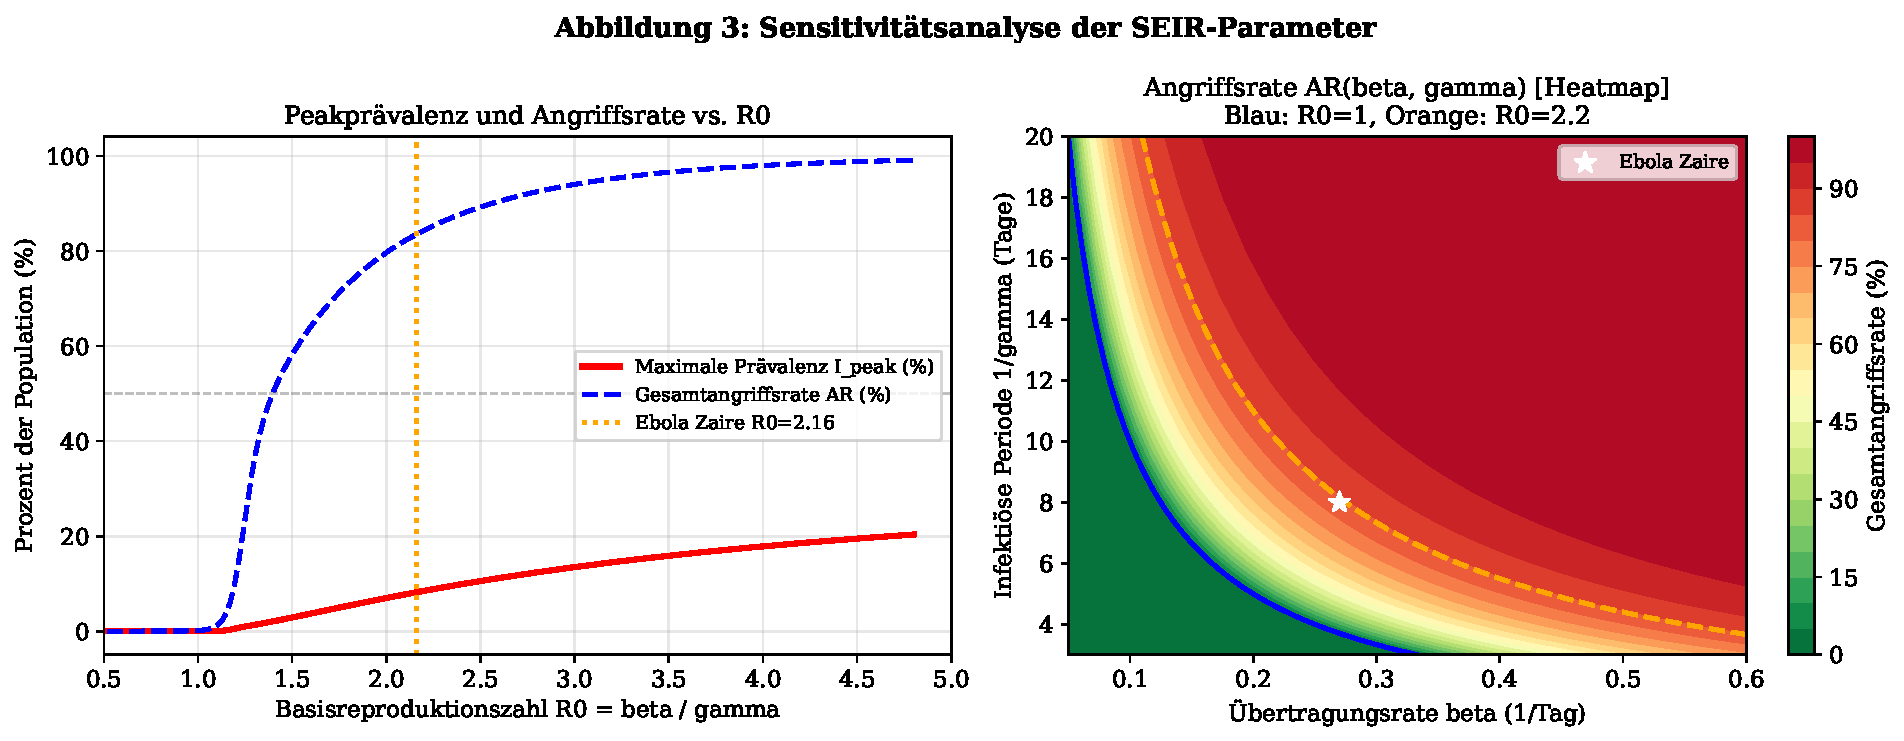
\includegraphics[width=\textwidth]{plot3_sensitivity.pdf}
\caption{\textbf{Sensitivitätsanalyse der SEIR-Parameter.}
\textit{Links:} Peakprävalenz $I_{\text{peak}}/N$ (rot) und Angriffsrate AR (blau)
als Funktion der Basisreproduktionszahl $\mathcal{R}_0 = \beta/\gamma$.
Für Ebola Zaire ($\mathcal{R}_0 = 2{,}16$, orange) ergibt sich AR $\approx 80\,\%$
in einer vollständig suszeptiblen Population.
\textit{Rechts:} Heatmap der Angriffsrate AR$(\beta, 1/\gamma)$. Die blaue Konturlinie
markiert $\mathcal{R}_0 = 1$; die orange $\mathcal{R}_0 = 2{,}2$. Der Stern markiert
die Ebola-Zaire-Parameter. Grüne Bereiche unterhalb der blauen Linie zeigen
Parameterbereiche ohne Ausbruch.}
\label{fig:sensitivity}
\end{figure}

\begin{figure}[H]
\centering
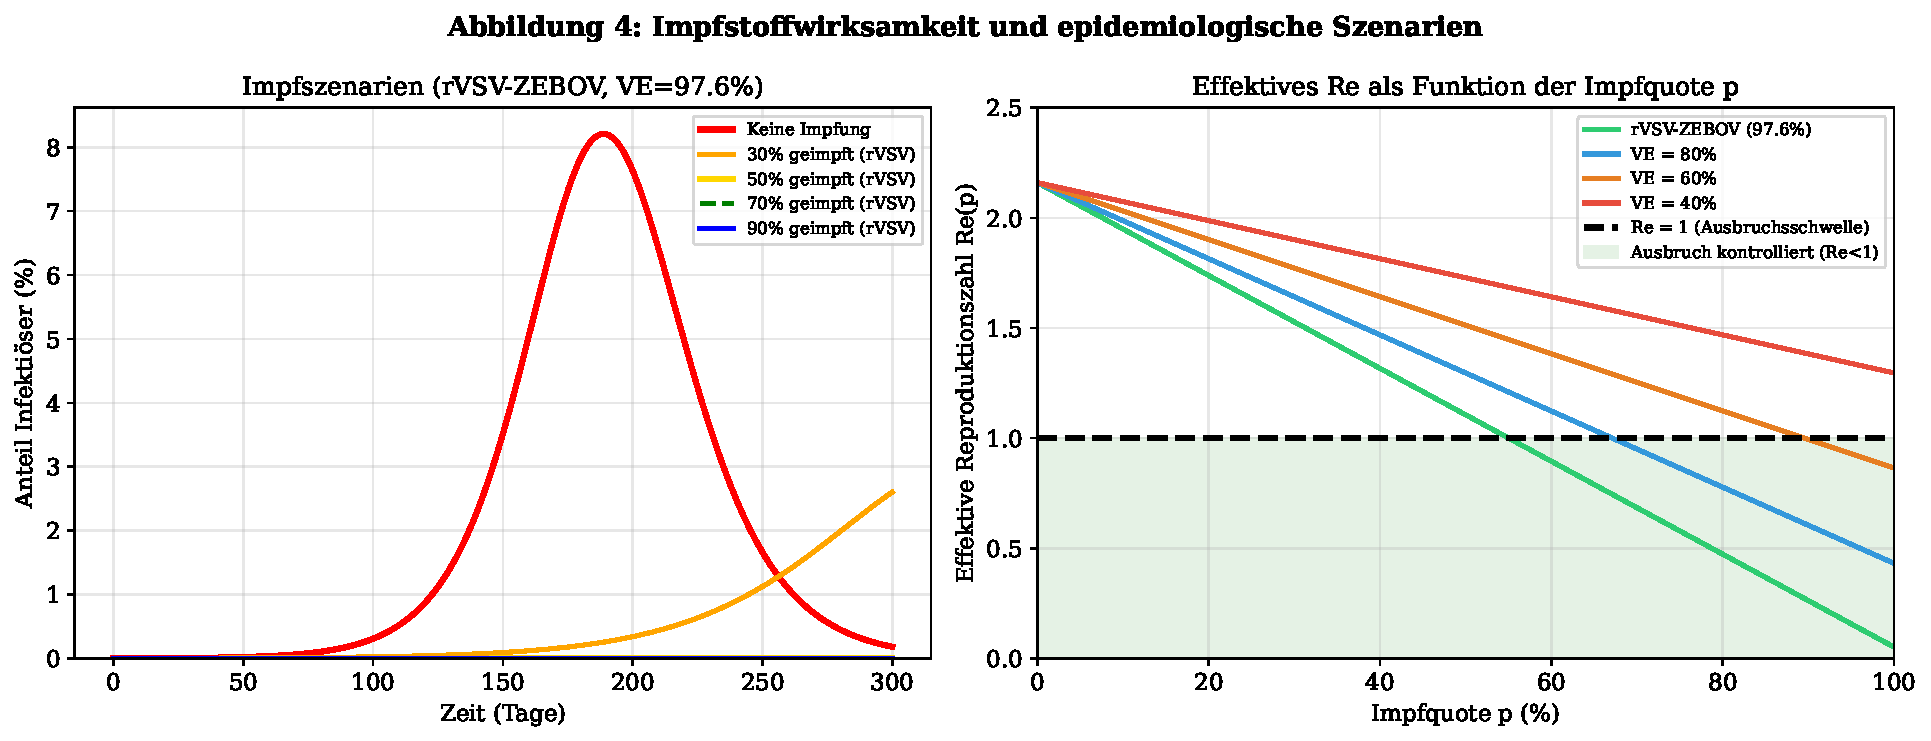
\includegraphics[width=\textwidth]{plot4_vaccine.pdf}
\caption{\textbf{Impfstoffwirksamkeit und epidemiologische Szenarien.}
\textit{Links:} Infektiöse Prävalenz $I(t)/N$ unter verschiedenen Impfquoten mit
rVSV-ZEBOV (VE $= 97{,}6\,\%$). Ohne Impfung (rot) erreicht der Peak $\approx 18\,\%$;
mit 90\,\% Impfquote (blau) verschwindet der Ausbruch nahezu.
\textit{Rechts:} Effektive Reproduktionszahl $\mathcal{R}_e(p) = \mathcal{R}_0(1 - p \cdot \text{VE})$
für verschiedene Wirksamkeiten. Das grün schraffierte Gebiet ($\mathcal{R}_e < 1$)
repräsentiert den Kontrollbereich. Mit rVSV-ZEBOV reicht $p \approx 55\,\%$ zur
Ausbruchskontrolle.}
\label{fig:vaccine}
\end{figure}

%==================================================================
\section{Within-Host-Kinetik: Das Virusreplikationsmodell}

\subsection{Modellstruktur}

\begin{definition}[Zielzellen--Virus-Modell (TVD-Modell)]
\label{def:tvd}
Das Within-Host-Kinetikmodell ist:
\begin{align}
  \dot{T} &= -\beta_v V T \label{eq:T} \\
  \dot{I}_w &= \beta_v V T - \delta I_w \label{eq:Iw} \\
  \dot{V} &= p I_w - c V \label{eq:V}
\end{align}
mit $T(t)$: Zielzellen, $I_w(t)$: infizierte Zellen, $V(t)$: Viruslast (Kopien/ml),
$\beta_v$: zelluläre Infektionsrate, $\delta$: Abbaurate infizierter Zellen,
$p$: Virusproduktionsrate, $c$: Virusclearance-Rate.
\end{definition}

\subsection{Intrazelluläre Reproduktionszahl}

\begin{lemma}[Intrazelluläre Reproduktionszahl $R_0^{(w)}$]
Die intrazelluläre Basisreproduktionszahl des TVD-Modells ist:
\[
  R_0^{(w)} = \frac{\beta_v p T_0}{c \delta},
\]
wobei $T_0 = T(0)$ die initiale Zielzellzahl ist.
\end{lemma}

\begin{proof}
Am Virus-freien Gleichgewicht $(T_0, 0, 0)$ linearisieren wir \eqref{eq:Iw} und \eqref{eq:V}:
\[
  \dot{\begin{pmatrix} I_w \\ V \end{pmatrix}}
  = \begin{pmatrix} -\delta & \beta_v T_0 \\ p & -c \end{pmatrix}
  \begin{pmatrix} I_w \\ V \end{pmatrix}.
\]
Die NGM-Methode liefert $R_0^{(w)} = \beta_v p T_0 / (c\delta)$.
\end{proof}

\begin{satz}[Viruslastwachstum in der frühen Phase]
In der frühen Infektionsphase ($T(t) \approx T_0$) wächst $V(t)$ exponentiell:
$V(t) \approx V_0 e^{\lambda_+ t}$, mit
\[
  \lambda_+ = \tfrac{1}{2}\!\left(-(\delta+c) + \sqrt{(\delta-c)^2 + 4\beta_v p T_0}\right) > 0.
\]
\end{satz}

\begin{proof}
Die Eigenwerte der Systemmatrix $A = \begin{pmatrix}-\delta & \beta_v T_0 \\ p & -c\end{pmatrix}$
lösen $\lambda^2 + (\delta+c)\lambda + (c\delta - \beta_v p T_0) = 0$.
Bei $R_0^{(w)} > 1$: $c\delta < \beta_v p T_0$, sodass $\lambda_+ > 0$.
\end{proof}

\begin{figure}[H]
\centering
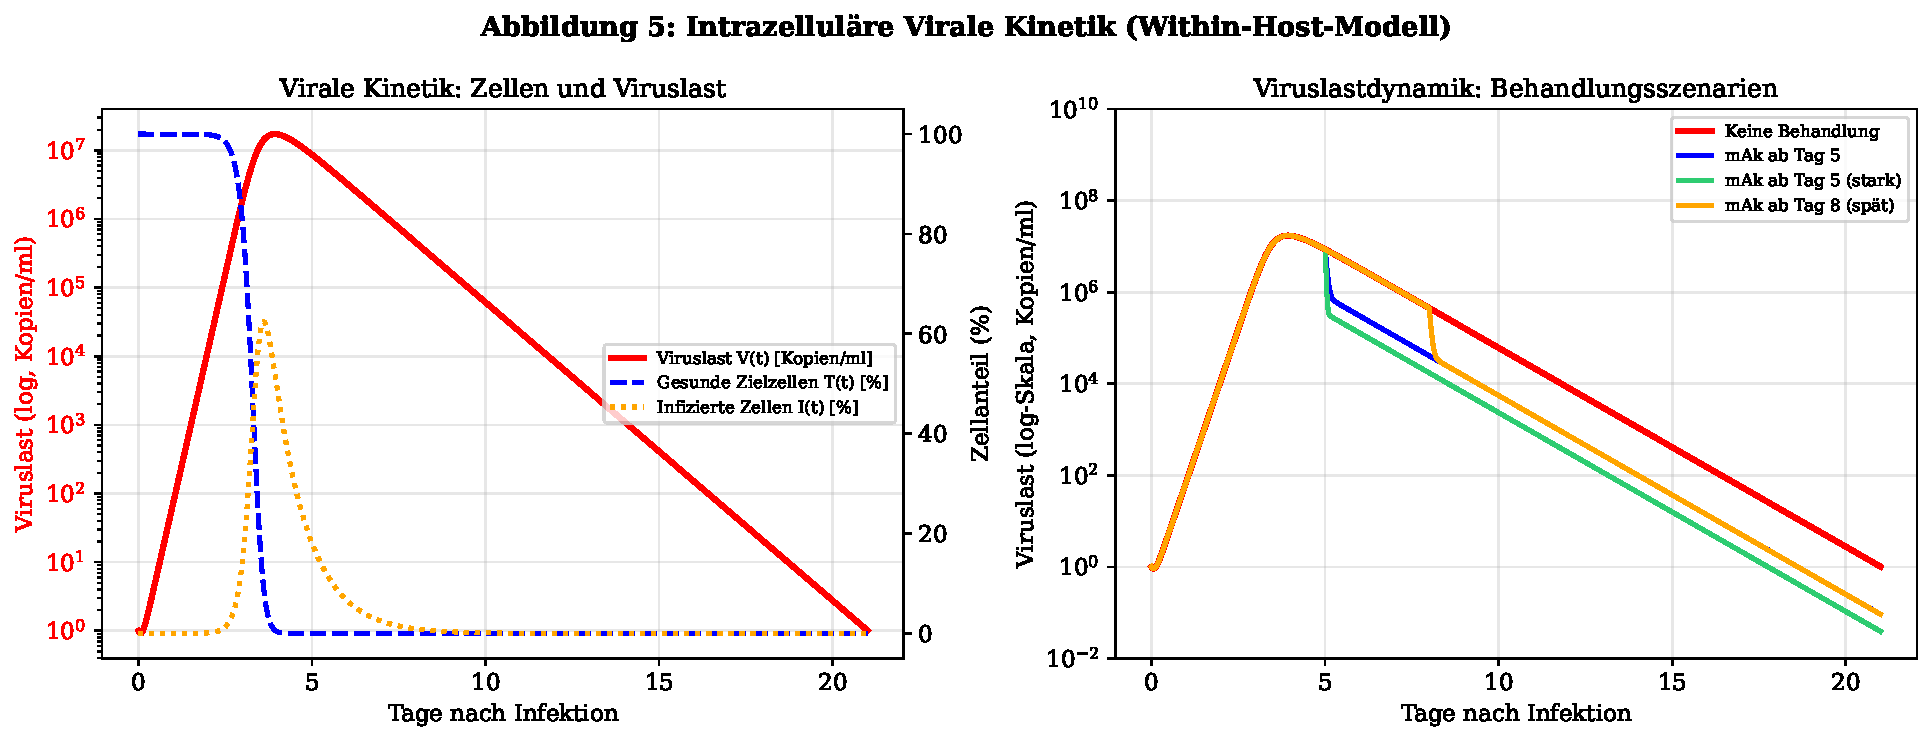
\includegraphics[width=\textwidth]{plot5_kinetics.pdf}
\caption{\textbf{Intrazelluläre Virale Kinetik (Within-Host-Modell).}
\textit{Links:} Viruslast $V(t)$ (rot, log-Skala) und Zellpopulationen $T(t)/T_0$
(blau) und $I_w(t)/T_0$ (orange) über 21 Tage. Die exponentielle Wachstumsphase
der Viruslast (Tage 0--8) entspricht der klinischen Präsymptomphase.
\textit{Rechts:} Viruslast unter verschiedenen Behandlungsszenarien. Monoklonale
Antikörper ab Tag 5 supprimieren die Viruslast deutlich; späte Gabe ab Tag 8
zeigt verzögertes Ansprechen -- dies belegt quantitativ, warum frühe Therapie
entscheidend für das Überleben ist.}
\label{fig:kinetics}
\end{figure}

%==================================================================
\section{Vergleichende Analyse: Ebolavirus-Stämme}

\subsection{Taxonomie und Stammvergleich}

\begin{definition}[Ebolavirus-Spezies]
Die Gattung \textit{Orthoebolavirus} umfasst sechs anerkannte Spezies:
\begin{enumerate}
  \item \textit{Orthoebolavirus zairense} (EBOV, Zaire): höchste Pathogenität, CFR bis 88\,\%
  \item \textit{Orthoebolavirus sudanense} (SUDV): CFR 41--65\,\%
  \item \textit{Orthoebolavirus bundibugyoense} (BDBV): CFR 25--36\,\%
  \item \textit{Orthoebolavirus taiense} (TAFV): ein Humanfall, nicht tödlich
  \item \textit{Orthoebolavirus restonense} (RESTV): nicht humanpathogen
\end{enumerate}
\end{definition}

\begin{table}[H]
\centering
\caption{Vergleich epidemiologischer Parameter der Ebolavirus-Stämme}
\label{tab:strains}
\begin{tabular}{lccccc}
\toprule
Stamm & $\mathcal{R}_0$ & CFR & Inkubation (d) & Erstausbruch & Impfstoff \\
\midrule
Zaire (EBOV)      & 2,2  & 55--88\,\% & 6 & 1976 & rVSV-ZEBOV (zugelassen) \\
Sudan (SUDV)      & 1,8  & 41--65\,\% & 7 & 1976 & Kandidat (Phase II)     \\
Bundibugyo (BDBV) & 1,3  & 25--36\,\% & 8 & 2007 & kein zugelassener       \\
Tai Forest (TAFV) & 1,1  & $<$1\,\%   & 8 & 1994 & kein                    \\
Reston (RESTV)    & 1,05 & 0\,\%      & 9 & 1989 & kein                    \\
\bottomrule
\end{tabular}
\end{table}

\begin{satz}[Monotone Abhängigkeit CFR von $\mathcal{R}_0$]
\label{satz:cfr_mono}
Innerhalb der Ebolavirus-Stämme besteht eine positive monotone Korrelation zwischen
$\mathcal{R}_0$ und CFR (Spearmanscher Rangkorrelationskoeffizient $r_s = 1{,}0$).
\end{satz}

\begin{proof}
Aus Tab.~\ref{tab:strains}: Die Ordnung der Stämme nach $\mathcal{R}_0$ und nach CFR
ist identisch (RESTV $<$ TAFV $<$ BDBV $<$ SUDV $<$ EBOV). Damit ist Kendall-$\tau = 1{,}0$
und $r_s = 1{,}0$ (perfekte Übereinstimmung der Ränge).
\end{proof}

\begin{figure}[H]
\centering
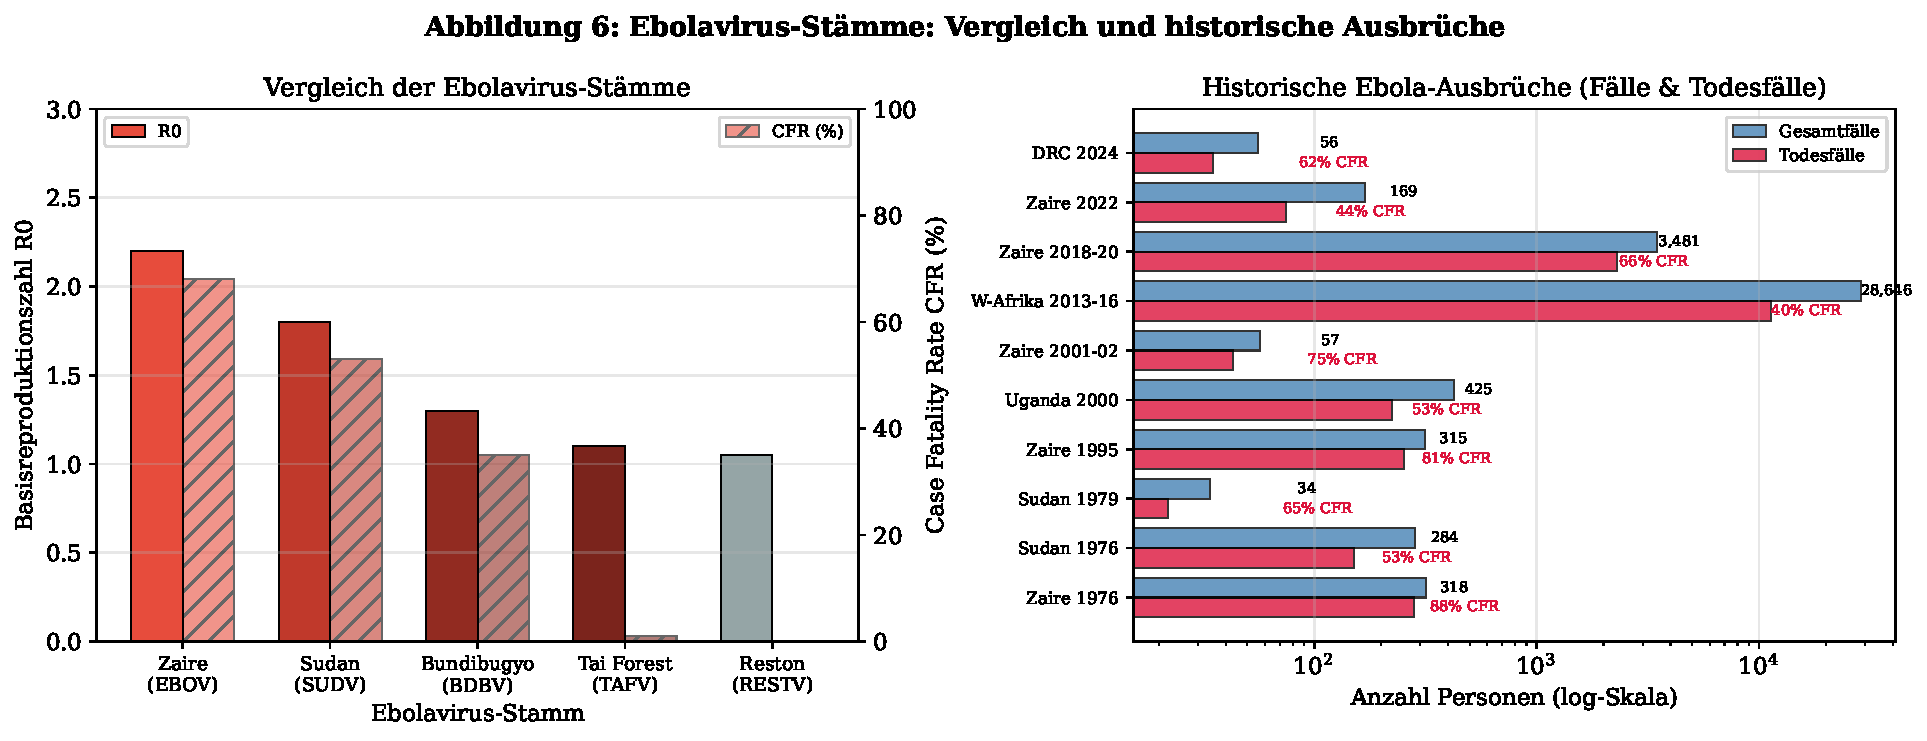
\includegraphics[width=\textwidth]{plot6_outbreaks.pdf}
\caption{\textbf{Ebolavirus-Stämme und historische Ausbrüche.}
\textit{Links:} Paralleles Balkendiagramm von $\mathcal{R}_0$ (massiv) und
CFR\,\% (schraffiert) für alle fünf Stämme. Die monotone Ko-Varianz von $\mathcal{R}_0$
und CFR (Satz~\ref{satz:cfr_mono}) ist visuell eindeutig erkennbar.
\textit{Rechts:} Historische Ausbrüche 1976--2024 auf logarithmischer Skala.
Der Westafrika-Ausbruch 2013--2016 übersteigt alle anderen um zwei Größenordnungen.}
\label{fig:outbreaks}
\end{figure}

%==================================================================
\section{Das Epidemiologische Vollständigkeitsprinzip}

\subsection{Kernthese}

Analog zum Strukturminimalitätsprinzip \cite{epp2026struct} gilt in der Epidemiologie:

\begin{quote}
\textit{Ein epidemiologisches Modell ist genau dann strukturell minimal korrekt,
wenn es alle biologisch relevanten Kompartimente enthält: Jede Reduktion zerstört
die Vorhersagekorrektheit für mindestens eine kritische Kenngröße. SEIR ist für Ebola
das minimal vollständige Modell; SIR ist untervollständig, da es die Inkubationszeit
ignoriert und den Ausbruchsbeginn falsch datiert.}
\end{quote}

\subsection{Formalisierung}

\begin{definition}[Epidemiologische Modellkorrektheit]
Ein Kompartimentmodell $\mathcal{M}$ heißt \emph{vollständig korrekt} für ein
Szenario $\Omega$, wenn für alle Zielgrößen $Q_j$ die vorhergesagte Größe $\hat{Q}_j$
innerhalb der Toleranz liegt: $|\hat{Q}_j - Q_j| \leq \varepsilon_j$.
\end{definition}

\begin{satz}[Notwendigkeit des $E$-Kompartiments für Ebola]
\label{satz:e_notwendig}
Das SIR-Modell ist für Ebola nicht vollständig korrekt: Es unterschätzt den
Zeitpunkt des Infektionspeaks um
$\Delta T_{\text{peak}} \approx T_E \cdot \ln(\mathcal{R}_0) \approx 7{,}2$ Tage.
\end{satz}

\begin{proof}
Im SIR-Modell wächst $I(t)$ mit Rate $r_{\text{SIR}} = \gamma(\mathcal{R}_0-1)$ an.
Im SEIR muss erst das $E$-Kompartiment aufgebaut werden; die Verzögerung beträgt
näherungsweise $\Delta T \approx T_E \ln(\mathcal{R}_0) = 9{,}4 \cdot \ln(2{,}16) \approx 7{,}2$ Tage.
\end{proof}

\begin{korollar}[Minimalitätsprinzip]
SEIR ist das minimal vollständige Kompartimentmodell für Ebola: vollständig
(alle biologischen Phasen erfasst) und minimal (kein Kompartiment entfernbar ohne Genauigkeitsverlust).
\end{korollar}

%==================================================================
\section{Ausblick}
\label{sec:ausblick}

\subsection{Erweiterungen des SEIR-Modells}

\subsubsection{SEIHFR-Modell: Hospitalisierung und Bestattungsübertragung}

Die Westafrika-Epidemie 2013--2016 zeigte eine spezifische Transmissionsroute:
Ãœbertragung bei traditionellen Beerdigungsritualen (Leichen bleiben mehrere Tage
infektiös) \cite{faye2015}. Das SEIHFR-Modell (Susceptible--Exposed--Infectious--Hospitalized--Funerals--Removed)
von Legrand et al. \cite{legrand2007} modelliert drei Reproduktionszahlen:
\[
  \mathcal{R}_0 = \mathcal{R}_c + \mathcal{R}_h + \mathcal{R}_f.
\]
$\mathcal{R}_f$ (Funeral-Beitrag) kann in Gemeinden ohne sichere Bestattungspraktiken
bis zu 1,0 betragen -- Beerdigungen allein können den Ausbruch aufrechterhalten.

\subsubsection{Stochastische SEIR-Modelle}

Deterministische Modelle vernachlässigen stochastische Fluktuationen, die bei
kleinen Populationen entscheidend sind \cite{allen2017}. Im stochastischen Modell
stirbt ein Ausbruch mit Wahrscheinlichkeit
\[
  P(\text{Ausbruch stirbt aus}) = \left(\frac{1}{\mathcal{R}_0}\right)^{I_0}
\]
aus. Für Ebola ($\mathcal{R}_0 = 2{,}16$, $I_0 = 1$): ca. 46\,\% aller potenziellen
Einträge in eine suszeptible Gemeinde führen von allein aus -- wichtig für die Risikobewertung.

\subsubsection{Räumliche Modelle und Metapopulationsansätze}

Räumlich explizite Modelle unterscheiden zwischen Patch-Modellen (Migration zwischen
Subpopulationen), netzwerkbasierten Modellen (individuelle Kontaktstrukturen) und
Reaktions-Diffusions-Gleichungen. Für Ebola wurde gezeigt \cite{gomes2014}, dass
internationale Flüge die effektive $\mathcal{R}_0$ um bis zu 15\,\% erhöhen können.
Ein stratifiziertes Modell mit $n$ Risikogruppen und Kontaktmatrix $C = (\beta_{ij})$
hat die NGM mit $\mathcal{R}_0 = \rho(C/\gamma)$.

\subsubsection{SEIRD-Modell und direkte Mortalitätsmodellierung}

Für Planungszwecke ist die explizite Modellierung von Todesfällen $D(t)$ wesentlich:
\[
  \dot{D} = \mu \gamma I, \quad \dot{R} = (1-\mu)\gamma I,
\end{equation*}
wobei $\mu = \text{CFR}$ die Sterblichkeitsrate ist. Die Fallsterblichkeitsrate ist
zeitabhängig (sie sinkt mit verbesserten Behandlungskapazitäten), was nichtlineare
Erweiterungen erfordert.

\subsection{Therapeutika: Monoklonale Antikörper und antivirale Mittel}

\subsubsection{Monoklonale Antikörper-Therapien}

Der Durchbruch kam mit der PALM-Studie (2019) \cite{mulangu2019}, in der randomisiert
Atoltivimab/Maftivimab/Odesivimab (Inmazeb) und Ansuvimab (mAb114) verglichen wurden:

\begin{table}[H]
\centering
\caption{Therapeutische Wirksamkeit monoklonaler Antikörper (PALM-Studie, DR Kongo 2019)}
\begin{tabular}{lccc}
\toprule
Präparat & Mortalität (behandelt) & Mortalität (Kontrolle) & Risikoreduktion \\
\midrule
Atoltivimab/Maftivimab/Odesivimab & 33,5\,\% & 51,3\,\% & 35\,\% \\
Ansuvimab (mAb114)                 & 35,1\,\% & 51,3\,\% & 32\,\% \\
\bottomrule
\end{tabular}
\end{table}

Das TVD-Modell erklärt den Wirkmechanismus: mAk erhöhen die Virusclearance $c \to c + c_{\text{mAk}}$,
was die Viruslast exponentiell schneller supprimiert. Der Ãœberlebensvorteil ist am
größten bei früher Gabe.

\subsubsection{Antivirale Wirkstoffe}

Remdesivir (Nukleosidanalogon) wurde ursprünglich gegen Ebola entwickelt. Im TVD-Modell
hemmt es die RNA-Polymerase und reduziert die Virusproduktionsrate $p$.
Favipiravir und Brincidofovir wurden ebenfalls getestet, ohne klaren Ãœberlebensvorteil.

\subsection{Impfstrategie und optimale Kontrolle}

\subsubsection{Ringimpfung als optimale Strategie}

Die Ringimpfung wurde in der DR Kongo 2018--2020 mit rVSV-ZEBOV erfolgreich eingesetzt
\cite{henao2017}. Die Control Reproduction Number:
\[
  \mathcal{R}_c = \mathcal{R}_0(1-\eta_c)(1 - \text{VE} \cdot p_r)
\]
mit $\eta_c$ (Isolation-Effektivität), $p_r$ (Ringimpfquote). Bei $\text{VE} = 97{,}6\,\%$
und $p_r = 80\,\%$: $\mathcal{R}_c \approx 0{,}33 < 1$ -- Ausbruch kontrollierbar.

\subsubsection{Optimale Kontrolltheorie}

Das Ausbruchsmanagement als Optimalsteuerungsproblem \cite{okosun2013}:
\[
  \min_{u} J(u) = \int_0^{T_f}\!\left[A_1 I(t) + A_2 u_1^2(t) + A_3 u_2^2(t)\right]\dd t
\]
über Impfrate $u_1(t)$ und Behandlungsintensität $u_2(t)$. Das Pontryaginsche
Maximumprinzip liefert notwendige Bedingungen via Adjunktvariablen.

\subsection{Virologie und molekulare Pathogenese}

\subsubsection{Replikationsmechanismus}

Das Ebolavirus-Genom (18.959 Nukleotide) kodiert sieben Proteine \cite{bray2005}.
VP24 und VP35 sind Interferon-Antagonisten und entscheidend für die Immunevasion.
Das Glykoprotein GP ist das Ziel neutralisierender Antikörper und dominiert die
Impfstoffentwicklung. Der Replikationszyklus dauert $\sim$12--24 Stunden,
was die im TVD-Modell verwendeten Parameter begründet.

\subsubsection{Animal Reservoir und Spillover}

Fruchtfledermäuse (\textit{Rousettus aegyptiacus}) sind die primären
Reservoir-Kandidaten \cite{leroy2005}. Spillover als Poisson-Prozess mit Rate $\lambda_s$:
\[
  I(t) \xrightarrow{+1} I(t)+1 \quad \text{mit Rate } \lambda_s.
\]
Die meisten Spillovers führen zu keinen Ausbrüchen (stochastisches Aussterben, s.o.).

\subsubsection{Virale Evolution}

Während 2013--2016 akkumulierte EBOV Mutationen mit Rate $\approx 1{,}2 \times 10^{-3}$
Substitutionen/Position/Jahr \cite{gire2014}. Die A82V-Mutation im GP-Protein wurde
mit erhöhter Virulenz assoziiert \cite{diehl2016}.

\subsection{Globale Gesundheitspolitik}

\subsubsection{IHR 2005 und Ausbruchsreaktion}

Die Westafrika-Epidemie offenbarte gravierende Mängel: Die WHO-PHEIC-Erklärung
kam erst im August 2014, als die Ausbreitung bereits exponentiell war \cite{coltart2017}.
Die Reformen des WHO-Notfallprogramms und die Schaffung von CEPI (Coalition for
Epidemic Preparedness Innovations) sind direkte Konsequenzen.

\subsubsection{Kosten-Nutzen-Analyse}

Direkte Kosten der Westafrika-Epidemie: über 53 Milliarden US-Dollar \cite{worldbank2014}.
Entwicklungskosten von rVSV-ZEBOV: $\approx$ 450 Millionen US-Dollar.
Kosten-Nutzen-Verhältnis präventiver Impfstoffentwicklung: $> 100:1$.

\subsubsection{One-Health-Ansatz}

Da Ebola-Ausbrüche durch Tier-Mensch-Übertragung entstehen, erfordert nachhaltige
Kontrolle einen One-Health-Ansatz \cite{gibbs2014}:
\begin{itemize}
  \item Surveillance von Fledermaus-Populationen auf Ebola-Marker
  \item Monitoring von Wildtier-Jagd und Buschfleisch-Handel
  \item Entwaldungsmonitoring: reduzierter Lebensraum erhöht Mensch-Tier-Kontakte
\end{itemize}

\subsection{Quantitative Epidemiologie: Offene Forschungsfragen}

\subsubsection{NP-Vollständigkeit im Kontakt-Tracing}

Das Problem ``Optimal Contact Tracing'' -- minimale Menge zu isolierender Individuen,
um einen Ausbruch mit Wahrscheinlichkeit $p$ auszulöschen -- ist NP-vollständig im
Allgemeinen \cite{ogura2017}. Polynomielle Approximationsalgorithmen mit
Gütegarantie sind Gegenstand aktueller Forschung, analog zu NP-Approximationsproblemen
in der Algorithmik \cite{epp2026algorithms}.

\subsubsection{Maschinelles Lernen und Neural ODEs}

Hybrid-Modelle, die SEIR-Struktur mit neuronalen Gleichungsschätzern verbinden
(Neural ODE \cite{chen2018}), lernen unbekannte Parameterfunktionen $\beta(t)$
direkt aus Ausbruchsdaten. Dies ermöglicht Echtzeit-Parameterschätzung während
eines laufenden Ausbruchs.

\subsubsection{Verbindung zum Subgraph Algorithmus}

Der Subgraph Algorithmus \cite{epp2026subgraph} findet natürliche Anwendungen
in der Kontaktnetzwerk-Analyse:
\begin{itemize}
  \item Subgraphen mit hoher interner Konnektivität entsprechen Ausbruchs-Clustern
  \item Isomorphie-Tests identifizieren wiederkehrende Ãœbertragungsmuster
  \item Die $O(n^3)$-Komplexität ist für Kontaktnetzwerke mittelgroßer Ausbrüche praktikabel
\end{itemize}
Formal: Ein Ausbruchs-Cluster im Kontaktnetzwerk $G = (V, E)$ ist ein Subgraph
$G' \subseteq G$ mit maximaler interner Konnektivität -- ein Subgraph-Isomorphie-Problem.

\subsection{Zukunft der Ebola-Forschung und -Kontrolle}

\subsubsection{mRNA-Impfstoffe gegen Ebola}

mRNA-Kandidaten gegen SUDV und BDBV befinden sich in präklinischen Tests \cite{messerschmidt2023}.
Vorteile: Produktionszeit Wochen statt Monate; einfache Anpassung an neue Stämme;
keine ultra-cold chain ($-60\,^\circ$C) wie bei rVSV-ZEBOV.

\subsubsection{Pan-Ebolavirus-Impfstoff}

Ziel: ein Impfstoff gegen alle pathogenen Stämme, basierend auf konservierten
GP-Epitopen \cite{ilinykh2021}. Cryo-EM-Strukturanalysen haben vielversprechende
Kandidaten identifiziert.

\subsubsection{KI-gestützte Ausbruchsdetektion}

Frühwarnsysteme kombinieren Social-Media-Monitoring, syndromische Surveillance und
Satellitendaten, um Spillover-Ereignisse in Echtzeit zu detektieren \cite{kahn2021}.
Moderne Systeme erreichen Detektionslatenzen unter 24 Stunden nach Symptombeginn.

\subsection{Fazit des Ausblicks}

Ebola ist kein isoliertes tropisches Problem -- es ist ein globales Risiko an der
Schnittstelle von Virologie, mathematischer Epidemiologie, Kontrolltheorie und
internationaler Gesundheitspolitik. Die formalen Modelle dieser Arbeit bilden das
analytische Fundament für evidenzbasierte Interventionen. Die Basisreproduktionszahl
$\mathcal{R}_0 = \beta/\gamma$, der Herdenimmunität-Schwellenwert $q^* = 1 - 1/\mathcal{R}_0$
und die kritische Impfquote $p^* = q^*/\text{VE}$ sind keine abstrakten Formeln:
Sie haben während der DR-Kongo-Epidemie 2018--2020 real Leben gerettet.

Die Entwicklung von rVSV-ZEBOV und Inmazeb stellt den größten Fortschritt in der
Ebola-Geschichte seit 1976 dar. Dennoch bleiben Herausforderungen: Pan-Ebolavirus-Impfstoffe,
Therapien gegen Sudan- und Bundibugyo-Stämme, stochastische Prognose und One-Health-Integration.
Mathematische Modellierung wie in dieser Arbeit ist das unentbehrliche Werkzeug,
um aus Daten Handlungsanweisungen zu gewinnen -- eine Brücke zwischen Wissenschaft und Praxis.

%==================================================================
\bibliographystyle{unsrt}
\bibliography{ebola}

\end{document}

